\section{6. Ограниченность непрерывной на отрезке функции. Теорема Вейерштрасса о достижимости точных граней. Теорема о промежуточных значениях непрерывной функции. Непрерыность монотонной функции, отображающей промежуток на промежуток. Теорема об обратной функции. Равномерная непрерывность. Теорема Кантора о равномерной непрерывности. Экспонента и ее свойства. Второй замечательный предел. Сравнение асимптотического поведения функций, $O$--символика.}

    \begin{definition}
        Функция называется \textit{непрерывной} на $D$, если она непрерывна в каждой точке множества $D$.
    \end{definition}

    \begin{lemma}
        Если функция $f$ непрерывна на $[a, b]$, то она ограничена на $[a, b]$.
    \end{lemma}

    \begin{proof}
        Предположим, что $f$ не является ограниченной. Тогда для каждого $n \in \N$ найдется такое $x_{n} \in [a, b]$, что $|f(x_{n})| > n$. По теореме Больцано--Вейерштрасса $\{x_{n}\}$ имеет сходящуюся подпоследовательность, $x_{n_{k}} \to c$. Переходя в неравенстве $a \leq x_{n_{k}} \leq b$ к пределу при $k \to \infty$ или пользуясь замкнутостью $[a, b]$, получаем $c \in [a, b]$. Тогда по непрерывности $f(x_{n_{k}}) \to f(c)$, что приводит к противоречию, т.к. $\{f(x_{n_{k}})\}$ неограничена.
    \end{proof}

    \begin{theorem}{Вейерштрасс}\\
        Если функция $f$ непрерывна на $[a, b]$, то существуют $x_{m}, x_{M} \in [a, b]$, такие что $f(x_{M}) = \sup_{x \in [a, b]} f(x)$ и $f(x_{m}) = \inf_{x \in [a, b]} f(x)$.
    \end{theorem}

    \begin{proof}
        По определению супремума для каждого $n \in \N$ найдется такое $x_{n} \in [a, b]$, что $M - \frac{1}{n} < f(x_{n}) \leq M$ и, значит, $f(x_{n}) \to M$. По теореме Больцано--Вейерштрасса существует подпоследовательность $\{x_{n_{k}}\}$, $x_{n_{k}} \to x_{M}$. Тогда по непрерывности $f(x_{n_{k}}) \to f(x_{M})$. С другой стороны, $f(x_{n_{k}}) \to M$. В силу единственности предела $f(x_{M}) = M$.\\
        Доказательство для инфимума аналогично.
    \end{proof}

    \begin{lemma}
        Если функция $f$ непрерывна на $[a, b]$ и $f(a)f(b) < 0$, то существует такое $c \in (a, b)$, что $f(c) = 0$.
    \end{lemma}

    \begin{proof}
        Пусть $f(a) < 0 < f(b)$. Положим $[a_{1}, b_{1}] = [a, b]$. Если $f(\frac{a_{1} + b_{1}}{2}) = 0$, то $c = \frac{a_{1} + b_{1}}{2}$. Иначе положим
        \[[a_{2}, b_{2}] = \begin{cases}
            [a_{1}, \frac{a_{1} + b_{1}}{2}], \text{ если } f(\frac{a_{1} + b_{1}}{2}) > 0,\\
            [\frac{a_{1} + b_{1}}{2}, b_{1}], \text{ если } f(\frac{a_{1} + b_{1}}{2}) < 0.
        \end{cases}\]
        Разделим $[a_{2}, b_{2}]$ пополам и повторим процесс. Если на некотором шаге функция $f$ обнулится в середине отрезка, то точка $c$ найдена. Иначе будет построена стягивающаяся последовательность отрезков $\{[a_{n}, b_{n}]\}$, что $f(a_{n}) < 0 < f(b_{n})$. По теореме Кантора существует точка $c$ -- общая для всех отрезков $[a_{n}, b_{n}]$, причем $a_{n} \to c$ и $b_{n} \to c$. Тогда $f(c) \leq 0 \leq f(c)$, т.е. $f(c) = 0$.
    \end{proof}

    \begin{center}
        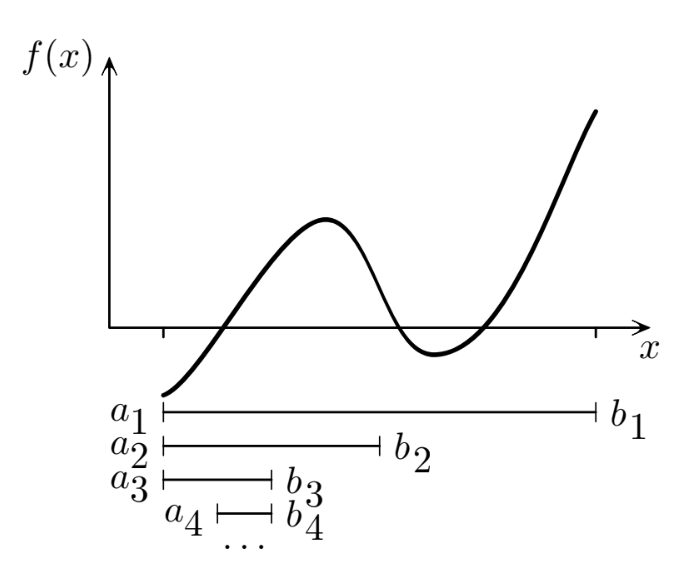
\includegraphics[width=0.33\textwidth]{none4.png}
    \end{center}

    \begin{theorem}{Коши о промежуточных значениях}\\
        Если функция $f$ непрерывна на $[a, b]$, то для любого числа $s$, лежащего между $f(a)$ и $f(b)$, найдется такое $c \in [a, b]$, что $f(c) = s$.
    \end{theorem}

    \begin{proof}
        Если $s$ совпадает с $f(a)$ или $f(b)$, то в качестве точки $c$ можно взять $a$ или $b$ соответственно. В противном случае рассмотрим функцию $g = f - s$. Функция $g$ непрерывна на $[a, b]$ и $g(a)g(b) < 0$. По лемме, существует $c \in (a, b)$, что $g(c) = 0$, т.е. $f(c) = s$.
    \end{proof}

    \begin{corollary}
        Если функция $f$ непрерывна на промежутке $I$, то $f(I)$ -- промежуток.
    \end{corollary}

    \begin{proof}
        Пусть $y_{1}, y_{2} \in f(I)$, тогда найдутся точки $x_{1}, x_{2} \in I$, такие что $y_{1} = f(x_{1})$ и $y_{2} = f(x_{2})$. Если $y_{1} \leq y \leq y_{2}$, то по теореме Коши существует точка $x \in [x_{1}, x_{2}]$, такая что $f(x) = y$. Так как $I$ -- промежуток, то $x \in I$ и, значит, $y \in f(I)$.
    \end{proof}

    \begin{lemma}
        Если функция $f$ монотонна на промежутке $I$ и $f(I)$ -- промежуток, то $f$ непрерывна на $I$.
    \end{lemma}

    \begin{proof}
        Пусть $f$ нестрого возрастает на $I$. Предположим, функция $f$ имеет разрыв в точке $c \in I$. Поскольку $f(c - 0) \leq f(c) \leq f(c + 0)$ (если $c$ -- концевая точка, то существет только один из односторонних пределов, для которого и проводятся рассуждения), то хотя бы одно из неравенств строгое и, значит, хотя бы один из интервалов $(f(c - 0), f(c))$ или $(f(c), f(c + 0))$ не пуст.\\
        Пусть интервал $J :=(f(c), f(c + 0))$ не пуст (случай непустого $(f(c-0), f(c))$ рассматривается аналогично). Тогда $f(t) \leq f(c)$ для любого $t \in I$, $t \leq c$, и $f(t) \geq \inf_{(c, \sup I)}f(x) = f(c + 0)$ для любого $t \in I$, $t > c$. Таким образом, интервал $J$ не пересекается с $f(I)$, но с обеих сторон имеются точки из $f(I)$. Это означает что $f(I)$ не является промежутком. 
    \end{proof}

    \begin{theorem}{Об обратной функции}\\
        Если функция $f: I \to \R$ строго монотонна и непрерывна на промежутке $I$, то $f(I)$ -- промежуток, $f$ -- биекция $I$ на $f(I)$ и обратная функция $f^{-1}: f(I) \to I$ также строго монотонна и непрерывна. 
    \end{theorem}

    \begin{proof}
        По следствию из теоремы Коши о промежуточных значениях, множество $J = f(I)$ является промежутком. Если $x_{1}, x_{2} \in I$ и $x_{1} \neq x_{2}$, то в силу строгой монотонности $f(x_{1}) \neq f(x_{2})$ и, значит, $f$ -- инъекция. Поэтому $f: I \to J$ -- биекция и существует обратная функция $f^{-1}: J \to I$.\\
        Пусть $f$ строго возрастает на $I$. Пусть $y_{1}, y_{2} \in J$ и $y_{1} < y_{2}$. Положим $x_{1} = f^{-1}(y_{1})$ и $x_{2} = f^{-1}(y_{2})$. Если $x_{1} \geq x_{2}$, то $y_{1} = f(x_{1}) \geq f(x_{2}) = y_{2}$, противоречие. Следовательно, $x_{1} < x_{2}$ и функция $f^{-1}$ строго возрастает. Так как $f^{-1}(J) = I$ -- промежуток, то по лемме функция $f^{-1}$ непрерывна на $J$.
    \end{proof}

    \begin{definition}
        Пусть функция $f$ определена на $E \subset \R$. Функция $f$ называется \textit{равномерно непрерывной} на $E$, если
        \[\forall \epsilon > 0 \ \exists \delta > 0 \ \forall x, x' \in E \ (|x - x'| < \delta \Rightarrow |f(x) - f(x')| < \epsilon).\]
    \end{definition}

    \begin{theorem}{Кантор}\\
        Если функция $f$ непрерывна на $[a, b]$, то она равномерно непрерывна на $[a, b]$.
    \end{theorem}

    \begin{proof}
        Пусть $f$ непрерывна, но не является равномерно непрерывной на $[a, b]$. Тогда 
        \[\exists \epsilon > 0 \ \forall \delta > 0 \ \exists x, x' \in [a, b] \ (|x - x'| < \delta \Rightarrow |f(x) - f(x')| \geq \epsilon).\]
        Полагая $\delta = \frac{1}{n}, \ n \in \N$, найдем соответствующие точки $x_{n}, x_{n}' \in [a, b]$, что $|x_{n} - x_{n}'| < \frac{1}{n}$ и $|f(x_{n}) - f(x_{n}')| \geq \epsilon$. По теореме Больцано--Вейерштрасса $\{x_{n}\}$ имеет сходящуюся подпоследовательность $\{x_{n_{k}}\}$, $x_{n_{k}} \to x_{0} \in [a, b]$. Поскольку $x_{n_{k}} - \frac{1}{n_{k}} \leq x_{n_{k}}' \leq x_{n_{k}} + \frac{1}{n_{k}}$, то $x_{n_{k}}' \to x_{0}$ по теореме о зажатой последовательности. Следовательно, $\lim_{k \to \infty}f(x_{n_{k}}) = \lim_{k \to \infty}f(x_{n_{k}}') = f(x_{0})$, что противоречит условию $|f(x_{n_{k}}) - f(x_{n_{k}}')| \geq \epsilon > 0$.
    \end{proof}

    \begin{definition}
        Функция $exp: \R \to \R$, $exp(x) = \lim_{n \to \infty}(1 + \frac{x}{n})^{n}$, называется \textit{экспонентой}.
    \end{definition}

    \begin{theorem}
        Для любого $x \in \R$ существует конечный $\lim_{n \to \infty} (1 + \frac{x}{n})^{n} = exp (x)$. Кроме того, $exp(x + y) = exp(x) \cdot exp(y)$ для всех $x, y \in \R$. 
    \end{theorem}
    
    \begin{proof}
        1) Докажем сходимость последовательности $a_{n} (x) = (1 + \frac{x}{n})^n$. Зафиксируем натуральное $m > |x|$. Тогда при $n \geq m$ верно $a_{n} (x) > 0$ и
        \[\frac{a_{n+1}(x)}{a_{n}(x)} = \frac{\left(1 + \frac{x}{n+1}\right)^{n+1}}{\left(1 + \frac{x}{n}\right)^{n}} = \left(1 + \frac{x}{n}\right)\left(\frac{(1 + \frac{x}{n+1})}{(1 + \frac{x}{n})}\right)^{n+1} = \left(1 + \frac{x}{n}\right)\left(1 - \frac{\frac{x}{n(n+1)}}{1 + \frac{x}{n}}\right)^{n+1}\]
        \\
        Выражение
        \[- \frac{\frac{x}{n(n+1)}}{(1 + \frac{x}{n})} > 0 \text{ при $x < 0$, и $\geq -1$ при $x \geq 0$}\]
        \\
        По неравенству Бернулли: $\frac{a_{n+1}(x)}{a_{n}(x)} \geq \left(1 + \frac{x}{n}\right)\left(1 - \frac{\frac{x}{n}}{1 + \frac{x}{n}}\right) = 1$, следовательно $\{a_{n}(x)\}$ нестрого возрастает при $n \geq m$.
        \\
        Т.к. $a_{n} (-x) \geq a_{m}(-x) \ \forall n \geq m$, то
        \[a_{n}(x) \cdot a_{n}(-x) = \left(1 + \frac{x}{n}\right)^{n}\left(1 - \frac{x}{n}\right)^{n} = \left(1 - \frac{x^{2}}{n^{2}}\right)^{n} \leq 1\]
        \\
        Следовательно, $a_{n}(x) \leq \frac{1}{a_{n}(-x)} \leq \frac{1}{a_{m}(-x)} \ \forall n \geq m$.
        \\
        Поэтому, последовательность $\{a_{n}(x)\}$ -- сходится.
        \\
        2) При $n > |x + y|$: 
        \[\left(1 + \frac{x}{n}\right)^{n} \left(1 + \frac{y}{n}\right)^{n} = \left(1 + \frac{x + y}{n} + \frac{xy}{n^{2}}\right)^{n} = \left(1 + \frac{x+y}{n}\right)^{n}\left(1 + \frac{\frac{xy}{n^{2}}}{1 + \frac{x + y}{n}}\right)^{n}\]
        Положим $\alpha_{n} = \frac{xy}{n + x + y}$.
        \\
        Для завершения доказательства достаточно показать, что $\lim_{n \to \infty} \left(1 + \frac{\alpha_{n}}{n}\right)^{n} = 1$.
        \\
        Выберем $N$ так, что $|\alpha_{n}| < 1$ при $n \geq N$.
        \\
        Поскольку $\left(1 + \frac{\alpha_{n}}{n}\right)^{n}\left(1 - \frac{\alpha_{n}}{n}\right)^{n} = \left(1 - \frac{\alpha_{n}^{2}}{n^{2}}\right)^{n} \leq 1$, по н-ву Бернулли при $n \geq N$:
        \[1 + \alpha_{n} \leq \left(1 + \frac{\alpha_{n}}{n}\right)^{n} \leq \frac{1}{\left(1 - \frac{\alpha_{n}}{n}\right)^{n}} \leq \frac{1}{1 - \alpha_{n}}\]
        $\Rightarrow \text{по теореме о зажатой последовательности } \lim_{n \to \infty} \left(1 + \frac{\alpha_{n}}{n}\right)^{n} = 1$.
    \end{proof}

    \begin{lemma} \ \\
        \begin{enumerate}
            \item $exp(x) \geq 1 + x \ \forall x \in \R$;
            \item $exp(x) \leq \frac{1}{1 - x} \ \forall x < 1$.
        \end{enumerate}
    \end{lemma}

    \begin{proof}
        Зафиксируем такой номер $N$, что $\frac{x}{N} \geq -1$. Тогда $(1 + \frac{x}{n})^{n} \geq 1 + x$ при всех $n \geq N$. Переходя к пределу при $n \to \infty$, получаем первое неравенство.\\
        Из пункта (1) следует, что $exp(-x) \geq 1 - x > 0$ при $x < 1$. Откуда, учитывая, что $exp(-x) = \frac{1}{exp(x)}$, получаем второе утверждение.
    \end{proof}

    \begin{theorem}
        Функция $exp$ непрерывна, строго возрастает и отображает $\R$ на $(0, +\infty)$.
    \end{theorem}

    \begin{proof}
        По лемме, для всех $x < 1$ имеют места неравенства $1 + x \leq exp(x) \leq \frac{1}{1 - x}$, откуда $\lim_{x \to 0}exp(x) = 1$. Теперь 
        \[\forall a \in \R \ \lim_{x \to a}exp(x) = \lim_{t \to 0}exp(t + a) = \lim_{t \to 0}(exp(a) \cdot exp(t)) = exp(a),\]
        что доказывает непрерывность экспоненты в точке $a$.\\
        Пусть $x, y \in \R$ и $x < y$. Тогда по лемме имеем
        \[exp(y) - exp(x) = \left(exp(y - x) - 1\right) \cdot exp(x) \geq (y - x) exp(x) > 0.\]
        Следовательно, функция $exp$ строго возрастает.\\
        По лемме $\lim_{x \to +\infty} exp(x) = +\infty$ и $\lim_{x \to -\infty} exp(x) = \lim_{x \to +\infty} exp(-x) = \lim_{x \to +\infty} \frac{1}{exp(x)} = 0$. Поэтому $\sup_{\R}exp(x) = +\infty$ и $\inf_{\R} exp(x) = 0$. Учитывая непрерывность экспоненты, заключаем, что множество значений $exp(\R) = (0, +\infty)$.
    \end{proof}

    \begin{definition}
        \textit{Натуральным логарифмом} называется функция $\ln: (0, +\infty) \to \R$, обратная к $exp$.
    \end{definition}

    \begin{lemma}{Второй замечательный предел}\\
        $\lim_{x \to 0} \frac{e^{x} - 1}{x} = 1$. Кроме того, $\lim_{x \to 0} \frac{\ln(x + 1)}{x} = 1$, $\lim_{x \to 0} (1 + x)^{\frac{1}{x}} = e$.
    \end{lemma}

    \begin{proof}
        По лемме для всех $x < 1$ выполнено $1 + x \leq e^{x} \leq \frac{1}{1 - x}$ или $x \leq e^{x} - 1 \leq \frac{x}{1 - x}$. Откуда $1 \leq \frac{e^{x} - 1}{x} \leq \frac{1}{1 - x}$ при $0 < x < 1$ и $\frac{1}{1 - x} \leq \frac{e^{x} - 1}{x} \leq 1$ при $x < 0$. По свойству предела зажатой функции $\frac{e^{x} - 1}{x} \to 1$ при $x \to 0$.\\
        Для функций $g(y) = \frac{y}{e^{y} - 1}$ и $f(x) = ln(x + 1)$ композиция $(g\circ f)(x) = \frac{\ln(x + 1)}{x}$, поэтому $\lim_{x \to 0}g(f(x)) = \lim_{y \to 0}g(y) = 1$ по свойству предела композиции.\\
        Рассмотрим функцию $h$, где $h(x) = \frac{\ln(x + 1)}{x}$ при $x \neq 0$, и $h(0) = 1$. Согласно предыдущему пункту $h$ непрерывна в нуле. Тогда композиция $(exp\circ h)(x) = (1 + x)^{\frac{1}{x}}$ также непрерывна в нуле и, значит, $\lim_{x \to 0} (exp\circ h)(x) = e$.
    \end{proof}

    \begin{definition}
        Пусть $f, g: E \to \R$, $a$ -- предельная точка $E$. Если существуют $\alpha: E \to \R$ и $\delta > 0$, такие что $f(x) = \alpha(x)g(x)$ для всех $x \in \overset{o}{B_{\delta}}(a) \cap E$, и
        \begin{enumerate}
            \item функция $\alpha$ ограничена на $\overset{o}{B_{\delta}}(a) \cap E$, то говорят, что $f$ \textit{ограничена по сравнению с $g$} при $x \to a$, и пишут $f(x) = O(g(x))$ при $x \to a$.
            \item функция $\alpha(x) \to 0$ при $x \to a$, то говорят, что $f$ \textit{бесконечно мала по сравнению с $g$} при $x \to a$, и пишут $f(x) = o(g(x))$ при $x \to a$.
            \item функция $\alpha(x) \to 1$ при $x \to a$, то говорят, что $f$и $g$ \textit{эквивалентны} или \textit{асимптотически равны} при $x \to a$, и пишут $f(x) \sim g(x)$ при $x \to a$.
        \end{enumerate}
    \end{definition}

    \begin{note}
        Если $g(x) \neq 0$ в некоторой проколотой окрестности $a$, то 
        \begin{enumerate}
            \item $f(x) = O(g(x))$ при $x \to a$ $\lra$ $\exists M > 0 \ \exists \delta > 0 \ \forall x \in \overset{o}{B_{\delta}}(a) \cap E \ (|\frac{f(x)}{g(x)}| \leq M)$;
            \item $f(x) = o(g(x))$ при $x \to a$ $\lra$ $\lim_{x \to a}\frac{f(x)}{g(x)} = 0$ ;
            \item $f(x) \sim g(x)$ при $x \to a$ $\lra$ $\lim_{x \to a}\frac{f(x)}{g(x)} = 1$. 
        \end{enumerate}
        Необходимость условий очевидна. Для доказательства обратного утверждения достаточно положить $\alpha(x) = \frac{f(x)}{g(x)}$ на $\overset{o}{B_{\delta}}(a) \cap E$ и $\alpha(x) = 0$ на $E \setminus \overset{o}{B_{\delta}}(a)$.
    \end{note}

    \begin{note}
        Важно понимать, что $O(g)$ и $o(g)$ -- это классы функций, и знак равенства означает принадлежность этому классу. Поэтому все такие равенства читаются только слева направо. Например, $x^{2} = o(x)$ и $x^{3} = o(x)$ при $x \to 0$, но $x^{2} \neq x^{3}$.
    \end{note}

    \begin{lemma}
        При $x \to a$ справедливы формулы:
        \begin{enumerate}
            \item $o(f) \pm o(f) = o(f), \ O(f) \pm O(f) = O(f)$;
            \item $o(f) = O(f)$;
            \item $o(O(f)) = o(f), \ O(o(f)) = o(f)$;
            \item $o(f)\cdot O(g) = o(fg)$.
        \end{enumerate}
    \end{lemma}

    \begin{proof}
        Докажем (4). Пусть $u(x) = o(f(x))$ при $x \to a$, т.е. $u = \alpha f$ в некоторой проколотой окрестности точки $a$, и функция $\alpha(x) \to 0$ при $x \to a$. Пусть $v(x) = O(g(x))$ при $x \to a$, т.е. $v = \beta g$ в некоторой проколотой окрестности точки $a$, причем функция $\beta$ там ограничена. Тогда на пересечении окрестностей $uv = (\alpha \beta)(fg)$ и $(\alpha \beta)(x) \to 0$ при $x \to a$. Это означает, что $u(x)v(x) = o(f(x)g(x))$ при $x \to a$.\\
        Остальные утверждения проверяются аналогично.
    \end{proof}

    Установим свойства асимптотического равенства.

    \begin{lemma}
        Справедливы следующие утверждения:
        \begin{enumerate}
            \item $f(x) \sim g(x)$ при $x \to a$ $\lra$ $f(x) = g(x) + o(g(x))$;
            \item если $f(x) \sim \tilde f(x), \ g(x) \sim \tilde g(x)$ при $x \to a$, то $f(x)g(x) \sim \tilde f(x) \tilde g(x)$ и $\frac{f(x)}{g(x)} \sim \frac{\tilde f(x)}{\tilde g(x)}$ при $x \to a$;
            \item если $f(x) \sim g(x)$ при $x \to a$, то $\lim_{x \to a}f(x)$ и $\lim_{x \to a}g(x)$ существуют одновременно (в $\overline{\R}$), и если существуют, то равны.
        \end{enumerate}
    \end{lemma}

    \begin{proof}
        Пусть функции $\alpha$ и $\beta$ в некоторой проколотой окрестности точки $a$ связаны соотношением $\alpha(x) = 1 + \beta(x)$. Тогда (1) следует из равносильности условий $\alpha(x) \to 1$ и $\beta(x) \to 0$ при $x \to a$. Утверждения (2) доказываются аналогично. При этом следует учесть, что множества определения $\frac{f}{g}$ и $\frac{\tilde f}{\tilde g}$ имеют непустое пересечение, для которого $a$ является предельной точкой.\\
        Докажем (3). Пусть $f(x) = \alpha(x) g(x)$ в некоторой проколотой окрестности точки $a$ и $\alpha(x) \to 1$ при $x \to a$. Тогда по свойству локализации $\lim_{x \to a} f(x)$ существует одновременно с $\lim_{x \to a} \alpha(x) g(x)$, который существует одновременно с $\lim_{x \to a} g(x)$. В случае существования все три предела равны.
    \end{proof}